\documentclass[12pt, letterpaper]{article}
\usepackage{color}
\usepackage{listings,lstautogobble}
\lstset{
    language=python,
    keywordstyle=\color{blue}, % language keywords style
    autogobble=true,
    commentstyle=\color{red}, % comment style
    frame=single,
    breaklines=true,
    basicstyle=\ttfamily
}
\usepackage{setspace}
\setstretch{1.3} % increase line spacing a tad - it's hard to read at 1 with this font or something
\usepackage{graphicx}
\usepackage{enumitem} % lets us create the table and set the margins
\usepackage{caption} % lets us add a caption to the table
\usepackage[natbibapa]{apacite} % allows citing in modern APA format (apalike is from 1992 and predates webpages)
\usepackage{geometry} % allows setting page info
\usepackage{url} % allows setting the space around URLs 
\Urlmuskip=0mu plus 1mu % helps with URL wrapping in the bibliography
\setlist[enumerate, 1]{leftmargin=0pt} % don't want big margins on list
\geometry{margin=1in} % don't want big margins on anything
\title{Midterm}
\author{Charlotte Braswell}
\date{\today}
\begin{document}
\maketitle
\pagebreak
\begin{enumerate}
    \item \textbf{Discuss solar reflected bands and emitted bands from Chapter 7. Limit: 2-3 pages}

    \pagebreak
    \item Algorithm Design
    \begin{enumerate}
    \item \textbf{Design your own algorithms for the detection of green grass, water clouds, and urban-residential using the reflectance from Figure 1 and within .4-2.5.}
    With "green grass", the spectral response function is heavily driven by chlorophyll's highly absorptive nature in the visible spectrum. Chlorophyll is very absorptive in the blue and red portions of the visible spectrum; however, it is reflective in the green portion of the visible spectrum. Most important for chlorophyll is the red-edge region, which is a region around .7 micrometers where the reflectance experiences a very sharp change. Therefore, any problem approaching green grass must factor in the response at ~ .8 micrometers (starting at .7 micrometers).

    For green grass, the following approximate wavelengths would be great:
    \begin{itemize}
    \item .8 micrometers, sudden change in reflectance
    \item .55 micrometers, slightly reflective
    \item 2.2 micrometers, slightly reflective but very absorptive
    \end{itemize}
    The response at .8 micrometers will allow distinguishing water, soil, clouds, and urban-residential. The response at 2.2 micrometers will allow distinguishing sand and green grass. The response at .55 is the green band, where it experiences a slight increase. 
    \bigskip

    Water clouds have a similar response function to ice clouds; however, they are rather distinct from the other categories in the visible spectrum. They are very reflective in the visible spectrum and parts of the near infrared. Ice clouds are also called Cirrus clouds, and they are best differentiated 

    For water clouds, the following approximate wavelengths would be great:
    \begin{itemize}
    \item Anywhere from .4 to .7 micrometers, due to its' high reflectance.
    \item 1.4 micrometers.
    \end{itemize}
    The response at 1.4 micrometers  would allow some differentiation between water and ice clouds. The high reflectively of clouds will allow easily differentiating between water/ice clouds and other factors at .4-.7.

    Urban-residential is very absorptive in the visible spectrum. Similar to grass, it becomes more reflective in the near infrared, although it is not nearly as reflective. 

    For urban-residential, the following approximate wavelengths would be great:
    \begin{itemize}
    \item .8 micrometers
    \item 1.9 micrometers
    \end{itemize}
    Capturing at .8 will allow differentiating between water, soil, grass, and clouds. Capturing at 1.9 micrometers will allow allow additional distinguishing between sand, soil, water, and clouds.

    \item \textbf{Which MODIS bands can be employed for detecting water vapor clouds, dust, and smoke.}
    
    \item \textbf{If you were to add two additional solar reflected bands in the .4-2.5 micrometer spectrum for future instruments, which bands would you select and why?}

    \end{enumerate}

    \item \textbf{Explain the various methods employed to extract Sensor Data Records (SDRs) from Raw Data Records (RDRs). This is the transformation of Digital Numbers (DNs) into Radiance, Reflectance, and Bright Temperatures.}
    \bigskip

    Landsat stores imagery using a collection and level structure. With the two different types of collections, the required processing, formulas, and availability differ. Landsat's Collection 1 data is available from 1972 onward; however, collection 1 became ineligible to download from the USGS in December 2022. Landsat's collection 2 implements a "substantial improvement" in geolocation, digital elevation sources, calibration, and validation (\cite{usgs_landsat_collections}). Since the collection 2 process is available for download for all Landsat versions, Landsat 9 is only collection 2, and collection 1 is not available for download, I will only discuss algorithms and information concerning collection 2. 
    
    Landsat's collection 2 level 1 data is stored using Digital Numbers (DNs). Early versions of Landsat used the Thematic Mapper (TM) or Thematic Mapper Plus (ETM+) sensors, which used 8-bit DNs (0-255). Landsat 8 and 9 use the Operational Land Imager (OLI) and Thermal Infrared Sensor (TIRS), which use 16-bit DNs (0-65,536). Accompanying the download of landsat level-1 product, the metadata file (MTL) contains information about the band operations to convert DNs to Top of Atmosphere (TOA) radiance, TOA reflectance, or TOA Brightness Temperature. Depending on needs, the file is provided in json, txt, and xml. Within the MTL file, the file name of each band is explicitly typed, constants required to perform the operations on each band are listed, projection information, and other assorted image information. See Figure~\ref{fig:mtl_file} for an example of the constants to calculate Radiance on Band 1.
    \begin{center}
        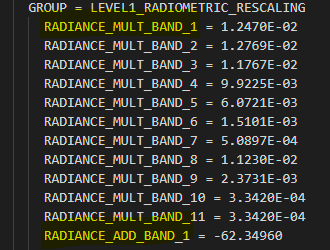
\includegraphics[scale=.7]{mtl_file.png}
        \captionof{figure}{Landsat MTL File, Highlighting Radiance Operations for Band 1}
        \label{fig:mtl_file}
    \end{center}
    
    The formula to convert from DNs ($Q_{cal}$) to TOA Radiance ($L_{\lambda}$) is $L_{\lambda} = M_LQ_{cal} + A_L$, where $M_p$ is the multiplicative rescaling factor and $A_p$ is the additive rescaling factor. Each band has the potential to have a different multiplicative rescaling and/or additive rescaling factor for each image. The syntax within the MTL file is the same, where the multiplicative factor is labeled RADIANCE\_MULT\_BAND\_X, and the additive factor is labeled RADIANCE\_ADD\_BAND\_X. In both cases, the \_X is substituted for the band number \cite{landsat_level1}.

    To convert DNs ($Q_{cal}$) to TOA Reflectance without correction for solar angle ($\rho_{\lambda}\prime$), the formula is $\rho_{\lambda}\prime = M_{\rho}Q_{cal} + A_{\rho}$. Similar to the above, $M_\rho$ is the multiplicative factor and $A_{\rho}$ is the additive factor. The MTL file is prefaced with REFLECTANCE\_MULTI\_BAND\_X or REFLECTANCE\_ADD\_BAND\_X. To calculate TOA planetary reflectance ($\rho_{\lambda}$) it is required to divide ($\rho_{\lambda}\prime$) by either $cos(\theta_{SZ})$ or $sin(\theta_{SE})$. $\theta_{SE}$ is the local sun elevation angle, and $\theta_{SZ}$ is the solar zenith angle \cite{landsat_level1}. In Python using Landsat Level-1 data for band 3 over East Tennessee, the below calculates the TOA reflectance:
    \begin{lstlisting}
        solar_correction = sin(float(mtl['IMAGE_ATTRIBUTES']['SUN_ELEVATION']) * pi/180)
        mp = float(mtl['LEVEL1_RADIOMETRIC_RESCALING']['REFLECTANCE_MULT_BAND_3'])
        ap = float(mtl['LEVEL1_RADIOMETRIC_RESCALING']['REFLECTANCE_ADD_BAND_3'])
        green_band = green.read(1)
        green_reflectance = mp*green_band + ap
        green_reflectance /= solar_correction
    \end{lstlisting}
    The sun elevation had to be converted from degrees to radians; however, the remainder of the formula was very straight forward.

    Lastly, to convert thermal band data to Top of Atmosphere Brightness Temperature ($T$), it is first required to calculate TOA Radiance ($L_{\lambda}$). The formula is then: $T = K_2/\ln(K_1/L_{\lambda} + 1)$. $K_1$ and $K_2$ and constants located in the MTL file as K1\_CONSTANT\_BAND\_X and K2\_CONSTANT\_BAND\_X. Notably, these constants are only available for thermal bands. In Landsat 8's case, this is bands 10 and 11, which are captured using TIRS versus OLI.

    \item \textbf{If Landsat-9 band 1 and 5 are not functional, which scientific products may be affected? How to generate those products with other measurements?}
    
    Landsat 9 captures data on 11 bands, using the Operational Land Imager (OLI) and Thermal Infrared Sensor (TIRS). Band 1 is the "coastal aerosol" band that captures data at a 30m resolution from .43 to .45 micrometers, and Band 5 is the "NIR" band that captures data at a 30m resolution from .85 to .88 micrometers \cite{landsat_9}. Reviewing Landsat's Common band combinations, it would affect Color Infrared (CIR), False Color (Vegetative Analysis), and Shortwave Infrared products \cite{landsat_9_band_combos}. Band 1 is primarily used for imaging shallow water and tracking aerosols like dust and smoke (\cite{nasa_landsat_bands}). Band 5 is commonly used for measuring plant health. Therefore if band 1 and 5 were to be degraded, removed, or otherwise negatively impacted, vegetation indices, aerosol products, and coastline products would also be negatively impacted. Since these measurements are needed for various scientific functions, it would not be advisable to not create an alternative implementation for products dependent on bands 1 and 5. For certain products, it may be possible to use a different band in-place of band 5 and 1. For instance, band 6 or band 2 could be used instead. However, it may also be possible to define the relationship typically observed with the bands 1 and 5 and other bands to impute the missing band 1/5 values. When Aqua's MODIS band 6 began experiencing failures, the Normalized Difference Snow Index (NDSI) was calculated using band 7 instead (\cite{modis_band_6}). However, it was also possible to use polynomial regression to calculate the reflectance values for Band 6 using the values in Band 7 with the formula: $R_{B6} = 1.6032R_{B7}^3 - 1.9458R_{B7}^2 + 1.7948R_{B7} + .012396$. In this formula $R_{B6}$ is the TOA reflectance value for band 6 and $R_{B7}$ is the TOA reflectance value for band 6. A similar process may be available for Landsat bands as well, depending on the relationship that may be exhibited between the bands. This would have to be fitted and validated before implementation, but it represents a viable alternative to replacing the bands with another band if a relationship exists.

\end{enumerate}
%\cite{qubook}
%\cite{modisfireatbd}
\pagebreak
\bibliographystyle{apacite}
\bibliography{refs}
\end{document}